\input{./preambule-sacha-utf8.ltx}
%
\usepackage{scrextend}
\usepackage[normalem]{ulem}  % Por barrer du texte 
\usetikzlibrary{matrix}

\addtokomafont{labelinglabel}{\sffamily}

\usepackage{colortbl} % xcolor est chargé automatiquement

\renewcommand{\CancelColor}{\red}

\newcommand{\intitule}[1]{{\huge \centerline {\textcolor{red}{#1\\ \bigskip}}}}
\newcommand{\vocabulaire}[1]{\textcolor{darkgreen}{#1}}
\newcommand{\Asavoir}[1]{\textcolor{red}{#1}}
\newcommand{\methode}[1]{\textcolor{blue}{#1}}

\newcommand{\TextSoulign}[2]{\textcolor{#1}{\underline{\textcolor{black}{#2}}}}

\newcommand{\marqueur}[1]{\tikz[remember picture]\node(#1){x};}

\newcolumntype{M}[1]{>{\raggedright}m{#1}}



\begin{document}

% \iffalse 
\intitule{Statistique : cours}

\begin{itemize}
\item le symbole $\Sigma$ signifie que l'on doit sommer.
\item on appelle $x_i$ les valeurs que peuvent prendre la chose que l'on étudie \vocabulaire{(le caractère)}
\item On appelle $n_i$ le nombre de fois où apparaît une valeur \vocabulaire{(les effectifs)}.
\end{itemize}

On appelle \Asavoir{moyenne} le nombre \Asavoir{$\overline{x}=\dfrac{\Sigma n_i x_i}{\Sigma n_i}$}

\bigskip 

\intitule{Statistique : exemple rédigé}

\begin{labeling}{Question}
\item [\underline{Énoncé :}] 
Les résultats au dernier contrôle de mathématiques de la classe de $4^{e}C$ sont : 

\centerline{\begin{tabular}{rrrrrrrrrr}
6 & 2 & 10 & 10 & 18 & 10 & 14 & 10 & 6 & 14 \\
14 & 14 & 2 & 6 & 14 & 10 & 6 & 14 & 14 & 6 \\
14 & 6 & 10 &  10 & 6 & 10 & 14 & 10 &  \\
\end{tabular}}

\item [\underline{Question :}] Déterminer la moyenne des notes au dernier contrôle de mathématiques. 
\end{labeling}

\begin{labeling}{Etape 1}
\item [\methode{\underline{Étape 1 :}}] \methode{On met les données dans un tableau}

\medskip
\centerline{\begin{tabular}{|l|c|c|c|c|c|}
\hline
Note obtenue & 2 & 6 & 10 & 14 & 18 \\
\hline
\multirow{3}{3cm}{Nombre d'élèves ayant obtenue cette note} &   &  &   &   &   \\
 & 2 & 7 & 9 & 9 & 1 \\
  &   &  &   &   &   \\
\hline
\end{tabular}}

\item [\methode{\underline{Étape 2 :}}] \methode{On identifie « qui sont » les $x_i$ et les $n_i$ ? }\\
On étudie des notes, les $x_i$ sont donc les notes obtenues et les $n_i$ les nombres d'élèves.

\item [\methode{\underline{Étape 3 :}}] \methode{On fait évoluer le tableau en le complétant de la manière suivante}\\(la partie supplémentaire est encadrée en bleu)

\medskip

\centerline{\setlength\doublerulesep{1pt}
 \doublerulesepcolor{blue}
 \begin{tabular}{|c|c|c|c|c|c||>{\columncolor{blue!20}\color{black}\bfseries}c||}
\hline
$x_i$ & 2 & 6 & 10 & 14 & 18 & $\Sigma$ \\
\hline
$n_i$ & 2 & 7 & 9 & 9 & 1 & 28\\
 \arrayrulecolor{blue}
\hline
\arrayrulecolor{blue} 
 \rowcolor{blue!20}$x_i n_i$ & 4 & 42 & 90 & 126 & 18 & 280 \\
\hline
 \arrayrulecolor{blue}
\end{tabular}}


\item [\methode{\underline{Étape 4 :}}] \methode{On calcule $\overline{x}$ (la moyenne)}

D'après le cours : $\overline{x} = \dfrac{\Sigma n_i x_i}{\Sigma n_i}$

On lit $\Sigma n_i x_i$ et $\Sigma n_i$ dans le tableau

On obtient = $\overline{x} = \dfrac{\Sigma n_i x_i}{\Sigma n_i} = \dfrac {280}{28} = 10 $

Donc la moyenne des notes des élèves est de $10/20$

\end{labeling}

\newpage 
%------------------------02 Géométrie --------------
                 
                 \intitule{Démontrer en géométrie : cours}
                 
\Asavoir{\underline {Méthode de rédaction}} 

\begin{labeling}{On sait que \ldots} 
\item  On sait que \ldots   \methode{On note les hypothèses qui permettent d'utiliser une propriété}
\item  or \ldots   \methode{On cite la propriété (ou son nom si elle en a un)}
\item  donc \ldots   \methode{On explique ce que l'on en conclut}
\end{labeling}

\Asavoir{Cette méthode permet de \underline{structurer} la démonstration.}

\bigskip 

 \intitule{Démontrer en géométrie : Exemple rédigé}
 
%------------------------03 Pythagore --------------
                 
                 \intitule{Théorème de Pythagore: cours} 
                 
\Asavoir{\Large 1) \underline {Énoncé du théorème}}    

\bigskip

\centerline {\begin{tabular}{l l} 
\multirow{5}{6cm}{\begin{tikzpicture}[line cap=round,line join=round,>=triangle 45,x=1.0cm,y=1.0cm]
\clip(-0.85,-0.85) rectangle (5.6,3.5);
\draw (0.475,0.) -- (0.475,0.475) -- (0.,0.475) -- (0.,0.) -- cycle; 
\draw  (0.,0.)-- (4.,0.) -- (0.,3.) -- (0.,0.);
\draw (0,1.5) node [left] {3};
\draw (2,0) node[below] {4};
\begin{scriptsize}
\draw [fill=black] (0.,0.) circle (1.5pt);
\draw (-0.2,0) node [below] {$A$};
\draw [fill=black] (4.,0.) circle (2.5pt);
\draw (4,-.1) node [below]{$B$};
\draw [fill=black] (0.,3.) circle (2.5pt);
\draw (-0.1,3) node [left] {$C$};
\end{scriptsize}
\end{tikzpicture}} & \\
                   & \\
                   & \methode{On a besoin}\\
                   & \methode{d'un triangle rectangle}\\
                   & \methode{et de 2 côtés connus}\\
\end{tabular}}  
                   
 \vspace*{2cm}           
                   
                   Dans un triangle rectangle, le carré de l'hypoténuse est égal à la somme des carrés des deux autres côtés, ici $BC^2 = AB^2 + AC^2$.
                   
 \bigskip 
 
 On a donc : 
 
 Triangle rectangle $\Longrightarrow BC^2 = AB^2 + AC^2$     
 
 
\bigskip 
 
 \Asavoir{\Large 2) \underline {Réciproque du théorème}}    

\bigskip

\centerline {\begin{tabular}{l l} 
\multirow{5}{6cm}{\begin{tikzpicture}[line cap=round,line join=round,>=triangle 45,x=1.0cm,y=1.0cm]
\clip(-0.85,-0.85) rectangle (5.6,3.5);
\draw (0.475,0.) -- (0.475,0.475) -- (0.,0.475) -- (0.,0.) -- cycle; 
\draw  (0.,0.)-- (4.,0.) -- (0.,3.) -- (0.,0.);
\draw (0,1.5) node [left] {3};
\draw (2,0) node[below] {4};
\draw (2,1.6) node[right] {5};
\begin{scriptsize}
\draw [fill=black] (0.,0.) circle (1.5pt);
\draw (-0.2,0) node [below] {$A$};
\draw [fill=black] (4.,0.) circle (2.5pt);
\draw (4,-.1) node [below]{$B$};
\draw [fill=black] (0.,3.) circle (2.5pt);
\draw (-0.1,3) node [left] {$C$};
\end{scriptsize}
\end{tikzpicture}} & \\
                   & \\
                   & \methode{On a besoin}\\
                   & \methode{de trois côtés connus}\\
                   & \methode{vérifiant l'égalité du théorème}\\
\end{tabular}}  
                   
 \vspace*{2cm}           
                   
Si $ABC$ est un triangle tel que  $BC^2 = AB^2 + AC^2$ alors $ABC$ est un triangle rectangle en $A$
                   
 \bigskip 
 
 On a donc : 
 
 $BC^2 = AB^2 + AC^2 \Longrightarrow $   triangle rectangle          
 
  
\newpage
 
 \Asavoir{\Large 3) \underline {Contraposée du théorème}}    

\bigskip

\centerline {\begin{tabular}{l l} 
\multirow{5}{6cm}{\begin{tikzpicture}[line cap=round,line join=round,>=triangle 45,x=1.0cm,y=1.0cm]
\clip(-0.85,-0.85) rectangle (5.6,3.5);
\draw (0.475,0.) -- (0.475,0.475) -- (0.,0.475) -- (0.,0.) -- cycle; 
\draw  (0.,0.)-- (4.,0.) -- (0.,3.) -- (0.,0.);
\draw (0,1.5) node [left] {3};
\draw (2,0) node[below] {4};
\draw (2,1.6) node[right] {7};
\begin{scriptsize}
\draw [fill=black] (0.,0.) circle (1.5pt);
\draw (-0.2,0) node [below] {$A$};
\draw [fill=black] (4.,0.) circle (2.5pt);
\draw (4,-.1) node [below]{$B$};
\draw [fill=black] (0.,3.) circle (2.5pt);
\draw (-0.1,3) node [left] {$C$};
\end{scriptsize}
\end{tikzpicture}} & \\
                   & \\
                   & \methode{On a besoin}\\
                   & \methode{de trois côtés connus}\\
                   & \methode{ne vérifiant pas l'égalité du théorème}\\
\end{tabular}}  
                   
 \vspace*{2cm}           
                   
Si $ABC$ est un triangle tel que  $BC^2 \neq AB^2 + AC^2$ alors $ABC$ n'est pas un triangle rectangle en $A$
                   
 \bigskip 
 
 On a donc : 
 
 $BC^2 \neq AB^2 + AC^2 \Longrightarrow $   triangle pas rectangle            
 
 %------------------------04 Exos Pythagore --------------
                 
                 \intitule{Théorème de Pythagore : Exemples rédigés} 
                 
\Asavoir{\Large 1) \underline {Théorème}}    

\bigskip   

\underline{Exemple 1 :} On cherche l'hypoténuse.

\centerline {\begin{tabular}{l l} 
\multirow{5}{6cm}{\begin{tikzpicture}[line cap=round,line join=round,>=triangle 45,x=1.0cm,y=1.0cm]
\clip(-0.85,-0.85) rectangle (5.6,3.5);
\draw (0.475,0.) -- (0.475,0.475) -- (0.,0.475) -- (0.,0.) -- cycle; 
\draw  (0.,0.)-- (4.,0.) -- (0.,3.) -- (0.,0.);
\draw (0,1.5) node [left] {3};
\draw (2,0) node[below] {4};
% \draw (2,1.6) node[right] {7};
\begin{scriptsize}
\draw [fill=black] (0.,0.) circle (1.5pt);
\draw (-0.2,0) node [below] {$A$};
\draw [fill=black] (4.,0.) circle (2.5pt);
\draw (4,-.1) node [below]{$B$};
\draw [fill=black] (0.,3.) circle (2.5pt);
\draw (-0.1,3) node [left] {$C$};
\end{scriptsize}
\end{tikzpicture}} & \\
                   & \\
                   &  Soit $ABC$ un triangle rectangle en $A$ tel que  \\
                   & $\qquad \left\{\begin{matrix}
                              AB=4\mathrm{cm}\\
                               AC=3\mathrm{cm}
                      \end{matrix}\right.$ \\
 & Déterminer la longueur du segment $[BC]$, \\
 & arrondie au millimètre s'il il y a lieu.\\
\end{tabular}}

\vspace*{2cm}
\begin{labeling}{On sait que} 
\item  [{\bf On sait que}]   $ABC$ est un triangle rectangle 
\item  [{\bf or}]    d'après le théorème de Pythagore, on a :

\centerline{\begin{tabular}{l>{$=\quad$}lcl}
            $BC^2$ & $AB^2 + AC^2$& \multirow{2}{.2cm}{${\textcolor{blue}{\left\downarrow\begin{matrix} \\ \end{matrix}\right.}}$}&\methode {On remplace par} \\
            $BC^2$ & $4^2 + 3^2$  & &\methode {ce que l'on connaît} \\
            $BC^2$ & $16 + 9$     & \multirow{3}{.2cm}{${\textcolor{blue}{\left\downarrow\begin{matrix} \\ \\ \end{matrix}\right.}}$}&\\
            $BC^2$ & $25$         & & \methode {On calcule}  \\
            $BC$ & $\sqrt{25}$    & &\\
            $BC$ & $5$            &  &\methode{On arrondit}\\
\end{tabular}}           
\item  [{\bf donc}]  $BC=5$ cm 
\end{labeling}

\newpage 

\underline{Exemple 2 :} On cherche la mesure d'un côté de l'angle droit

\centerline {\begin{tabular}{l l} 
\multirow{5}{6cm}{\begin{tikzpicture}[line cap=round,line join=round,>=triangle 45,x=1.0cm,y=1.0cm]
\clip(-0.85,-0.85) rectangle (5.6,3.5);
\draw (0.475,0.) -- (0.475,0.475) -- (0.,0.475) -- (0.,0.) -- cycle; 
\draw  (0.,0.)-- (4.,0.) -- (0.,3.) -- (0.,0.);
% \draw (0,1.5) node [left] {3};
\draw (2,0) node[below] {4};
\draw (2,1.6) node[right] {7};
\begin{scriptsize}
\draw [fill=black] (0.,0.) circle (1.5pt);
\draw (-0.2,0) node [below] {$C$};
\draw [fill=black] (4.,0.) circle (2.5pt);
\draw (4,-.1) node [below]{$A$};
\draw [fill=black] (0.,3.) circle (2.5pt);
\draw (-0.1,3) node [left] {$B$};
\end{scriptsize}
\end{tikzpicture}} & \\
                   & \\
                   &  Soit $ABC$ un triangle rectangle en $A$ tel que  \\
                   & $\qquad \left\{\begin{matrix}
                              AC=4\mathrm{cm}\\
                               AB=7\mathrm{cm} 
                      \end{matrix}\right.$ \\
 & Déterminer la longueur du segment $[BC]$, \\
 & arrondie au millimètre s'il il y a lieu.\\
\end{tabular}}

\vspace*{2cm}
\begin{labeling}{On sait que} 
\item  [{\bf On sait que}]   $ABC$ est un triangle rectangle en $C$ et que $AB = 4$cm et $AB=7$cm 
\item  [{\bf or}]    d'après le théorème de Pythagore, on a :

\centerline{\begin{tabular}{llcl}
            $AB^2 = AC^2 + BC^2$& \multirow{2}{.2cm}{${\textcolor{blue}{\left\downarrow\begin{matrix} \\ \end{matrix}\right.}}$}&\methode {On remplace par} \\
            $\;\;\;\; 7^2 = 4^2 + BC^2$  & &\methode {ce que l'on connaît} \\
           $BC^2 = 7^2 -4^2$     & \methode{$\downarrow$} & \methode {On isole l'inconnue}  \\ 
$BC^2 = 49 - 16 $  & \multirow{3}{.2cm}{${\textcolor{blue} {\left\downarrow\begin{matrix} \\ \\   \end{matrix}\right.}}$} &  \\
           $BC^2 = 33 $         & & \methode {On calcule}  \\
            $BC = \sqrt{33}$    & & \\
           $BC  \simeq 5,7$            & \methode{$\downarrow$} &\methode{On arrondit}\\
\end{tabular}}          
\item  [{\bf donc}]  $BC=5,7$ cm 
\end{labeling}


\bigskip 
                 
\Asavoir{\Large 2) \underline {Réciproque du théorème}}    

\bigskip   

\underline{Exemple:} On cherche à montrer que le triangle est rectangle. \\

Soit $ABC$ un triangle tel que $ \left\{\begin{matrix}
                              AB=5\mathrm{cm}\\
                               AC=13\mathrm{cm}\\
                               BC=12\mathrm{cm}
                      \end{matrix}\right.$ 

\bigskip                       
                      
\begin{tabular}{ll@{}ll}
 On a &     $AB^2 + BC^2\;$ & $=  5^2 + 12^2$ &  \\
      &              & $= 25 + 144 $ & \multirow{2}{2cm}{\methode{On vérifie en \underline{2 parties} }}\\
      &              & $=  169 $ & \\  
      &              &           &  \\
De plus & $AC^2$ & $= 13^2$  &  \multirow{2}{2cm}{\methode{ que l'égalité est vérifiée}}\\
        &        & $= 169$   & \\    
      &              &           & \\
Ainsi & $AC^2$ & $= AB^2 + BC^2 $ & \\                     
     \end{tabular}                    

\bigskip 

Donc, d'après la réciproque du théorème de Pythagore, le triangle $ABC$ est rectangle en $B$.                                
  
\newpage 
 
                  
\Asavoir{\Large 3) \underline {Contraposée du théorème}}    

\bigskip   

\underline{Exemple:} On cherche à montrer que le triangle n'est pas rectangle. \\

Soit $ABC$ un triangle tel que $ \left\{\begin{matrix}
                              AB=3,5\mathrm{cm}\\
                               AC=3,5\mathrm{cm}\\
                               BC=5\mathrm{cm} 
                      \end{matrix}\right.$ 

\bigskip                       
                      
\begin{tabular}{ll@{}ll}
 On a &     $AB^2 + AC^2\;$ & $=  3,5^2 + 3,5^2$ &  \\
      &              & $= 12,25 + 112,25 $ & \multirow{2}{2cm}{\methode{On vérifie en \underline{2 parties} }}\\
      &              & $=  24,5 $ & \\  
      &              &           &  \\
De plus & $BC^2$ & $= 5^2$  &  \multirow{2}{2cm}{\methode{ que l'égalité n'est pas vérifiée}}\\
        &        & $= 25$   & \\    
      &              &           & \\
Ainsi & $AC^2$ & $\neq AB^2 + BC^2 $ & \\                     
     \end{tabular}                    

\bigskip 

Donc, d'après la réciproque du théorème de Pythagore, le triangle $ABC$ n'est pas rectangle en $A$.                                
  
\newpage  

%------------------------05 Vitesse --------------
                 
                 \intitule{Vitesse, distance et temps : cours} 
                 
\Asavoir{
\begin{tabular}{l@{\hspace*{3cm}}l}
\underline{\Large Formules à retenir} & \begin{tabular}{l}
	$ v \longleftarrow$  vitesse \\
	$ d \longleftarrow$ distance \\
	$ t \longleftarrow$ temps \\
\end{tabular} \\
  & \\
 & $v = \dfrac{d}{t}$ \\
\end{tabular} 
}

\begin{labeling}{On en déduit que :} 
\item [On en déduit que :] \Asavoir{$d = v \times t$}
\item [et :] \Asavoir {$t = \dfrac{d}{v}$} 
\end{labeling}    

\medskip

Dans ces formules, le temps est exprimé en forme \Asavoir{décimale}.

\begin{labeling}[$\bullet$]{Remarques : }
\item [\underline{Remarques} : ] On utilise $v=\dfrac{d}{t}$ si on cherche la vitesse.   
\item [] On utilise $d=vt$ si on cherche la distance.   
\item [] On utilise $t=\dfrac{d}{v}$ si on cherche la temps.   
\end{labeling}

\bigskip
                   
                 \intitule{Vitesse, distance et temps} 

                 \centerline{\Asavoir{\large Exemples rédigés de trois types}}   

\medskip                     
                 
\Asavoir{\Large 1) On cherche la vitesse}    

\medskip  

Une personne roule à la même vitesse pendant 4 heures et parcourt 250 km. À quelle \underline{vitesse} roule-t-elle ? 

\begin{labeling}{On sait que}
\item [On sait que] $ d = 250$km et que $t=4$h 
\item [or] $v=\dfrac{d}{t}$ 
\item [donc] $v=\dfrac{d}{t} = \dfrac{250}{4}=62,5$
\end{labeling}

\smallskip

La personne roule à $62,5$km/h 

\medskip

\Asavoir{\Large 2) On cherche une distance}    

\medskip  

Une personne roule à 120km/h pendant 6 heures. Quelle \underline{distance} aura-t-elle parcourue ?  

\begin{labeling}{On sait que}
\item [On sait que] $ v = 120$ et que $t=6$ 
\item [or] $d=v\times t$ 
\item [donc] $d=vt=120\times6=720$
\end{labeling}

\smallskip

La personne aura parcourue $720$km
   
\medskip

\Asavoir{\Large 3) On cherche une durée}    

\medskip 

Une personne parcourt 480 km à la vitesse de 120 km/h. Combien de \underline{temps} cette personne a-t-elle roulé  ?  

\begin{labeling}{On sait que}
\item [On sait que] $ d = 480$ et que $v = 120$
\item [or] $t=\dfrac{d}{v}$ 
\item [donc] $t=\dfrac{d}{v} = \dfrac{480}{120} = 4$ 
\end{labeling}

\smallskip

La personne aura roulé 4 heures

\newpage

 %------------------------06 Trigonometrie --------------
                 
                 \intitule{Trigonométrie : cours} 
                 


\bigskip   

\newcolumntype{M}[1]{>{\raggedright}m{#1}}

\begin{tabular}{M{7cm}M{6cm}}
\Asavoir{\Large $ \bullet \quad  0 \leqslant \cos (x)  \leqslant 1$}    

\medskip 

\Asavoir{\Large $\bullet \quad  \cos(x) = \tfrac{adjacent}{hypothénuse} = \dfrac{OB}{OA}$ }    & 

\begin{tikzpicture}[line cap=round,line join=round,>=triangle 45,x=1.0cm,y=1.0cm, scale=.75]
\clip(-1,-1) rectangle (5.5,3.75);
\draw[color=darkgreen,fill={darkgreen!75},fill opacity=0.1] (4.,0.5) -- (3.5,0.5) -- (3.5,0.) -- (4.,0.) -- cycle; 
\draw [shift={(0.,0.)},color=darkgreen,fill={darkgreen!75},fill opacity=0.1] (0,0) -- (0.:0.6) arc (0.:36.85:0.6) -- cycle;
\draw (0.,0.)-- (4.,0.);
\draw (4.,0.)-- (4.,3.);
\draw (4.,3.)-- (0.,0.);
\draw [domain=-1.:5.5] plot(\x,{(-0.--3.*\x)/4.});
\draw [domain=-1.8:5.5] plot(\x,{(-0.-0.*\x)/4.});
\draw (0.7,0.3) node[right] {$\alpha$};
\begin{scriptsize}
\draw (0.,0.) circle (1pt);
\draw (0.15,-0.25) node {$O$};
\draw  (4.,0.) circle (1pt);
\draw (4,-.1) node[below]{$B$};
\draw (4.,3) circle (1pt);
\draw (4,3.2) node[left]{$A$};
\end{scriptsize}
\end{tikzpicture}
                    
\end{tabular} 
                    
$\hookrightarrow$ Par définition, \Asavoir{toujours} dans un triangle rectangle.                                    

\bigskip
                   
                 \intitule{Trigonométrie} 

                 \centerline{\Asavoir{\large Exemples rédigés de quatre types}}   

\bigskip                     
                 
\Asavoir{\Large \underline{Exemple 1 : } On cherche le cosinus}, ici de $\widehat{AOB}$    



\begin{tabular}{M{1.9cm}M{6cm}r}
\methode{On a besoin de 2 côtés} & 
\begin{tikzpicture}[line cap=round,line join=round,>=triangle 45,x=1.0cm,y=1.0cm, scale=.75]
\clip(-1,-1) rectangle (5.5,3.75);
\draw[color=darkgreen,fill={darkgreen!75},fill opacity=0.1] (4.,0.5) -- (3.5,0.5) -- (3.5,0.) -- (4.,0.) -- cycle; 
\draw [shift={(0.,0.)},color=darkgreen,fill={darkgreen!75},fill opacity=0.1] (0,0) -- (0.:0.6) arc (0.:36.85:0.6) -- cycle;
\draw (0.,0.)-- (4.,0.);
\draw (4.,0.)-- (4.,3.);
\draw (4.,3.)-- (0.,0.);
\draw [domain=-1.:5.5] plot(\x,{(-0.--3.*\x)/4.});
\draw [domain=-1.8:5.5] plot(\x,{(-0.-0.*\x)/4.});
\draw (0.7,0.3) node[right] {$\alpha$};
\begin{scriptsize}
\draw (0.,0.) circle (1pt);
\draw (0.15,-0.25) node {$O$};
\draw  (4.,0.) circle (1pt);
\draw (4,-.1) node[below]{$B$};
\draw (4.,3) circle (1pt);
\draw (4,3.2) node[left]{$A$};
\draw (2,1.6) node[left]{$5$};
\draw (2,0) node[below]{$4$};
\end{scriptsize}
\end{tikzpicture}
                  & \vocabulaire{On applique le cours} \\
\end{tabular}

\begin{labeling}{On sait que}
\item [On sait que] le triangle $AOB$ est rectangle en $B$
\item [or] $ \cos(\alpha) = \tfrac{adjacent}{hypothénuse} $ 
\item [donc] $\cos(\widehat{AOB}) = \dfrac{OB}{OA} = \dfrac{4}{5}$
\end{labeling}

\medskip                     
                 
\Asavoir{\Large \underline{Exemple 2 : } On cherche un angle}, ici l'angle $\widehat{AOB}$    



\begin{tabular}{M{2.5cm}M{6cm}M{6cm}}
\methode{On a besoin \\du cosinus \\de l'angle $\widehat{AOB}$ } & 
\begin{tikzpicture}[line cap=round,line join=round,>=triangle 45,x=1.0cm,y=1.0cm, scale=.75]
\clip(-1,-1) rectangle (5.5,3.75);
\draw[color=darkgreen,fill={darkgreen!75},fill opacity=0.1] (4.,0.5) -- (3.5,0.5) -- (3.5,0.) -- (4.,0.) -- cycle; 
\draw [shift={(0.,0.)},color=darkgreen,fill={darkgreen!75},fill opacity=0.1] (0,0) -- (0.:0.6) arc (0.:36.85:0.6) -- cycle;
\draw (0.,0.)-- (4.,0.);
\draw (4.,0.)-- (4.,3.);
\draw (4.,3.)-- (0.,0.);
\draw [domain=-1.:5.5] plot(\x,{(-0.--3.*\x)/4.});
\draw [domain=-1.8:5.5] plot(\x,{(-0.-0.*\x)/4.});
\draw (0.7,0.3) node[right] {$\alpha$};
\begin{scriptsize}
\draw (0.,0.) circle (1pt);
\draw (0.15,-0.25) node {$O$};
\draw  (4.,0.) circle (1pt);
\draw (4,-.1) node[below]{$B$};
\draw (4.,3) circle (1pt);
\draw (4,3.2) node[left]{$A$};
\draw (2,1.6) node[left]{$5$};
\draw (2,0) node[below]{$4$};
\end{scriptsize}
\end{tikzpicture}
                  & \vocabulaire{$\bullet$ On fait comme l'exemple 1\\
                                 $\bullet$ On utilise la calculatrice} \\
\end{tabular}

\begin{labeling}{On sait que}
\item [On sait que] le triangle $AOB$ est rectangle en $B$
\item [or] $ \cos(\alpha) = \tfrac{adjacent}{hypothénuse} $ 
\item [donc] $\cos(\widehat{AOB}) = \dfrac{OB}{OA} = \dfrac{4}{5}$
\item []     $\widehat{AOB} = \arccos \left(\dfrac{4}{5}\right)$
\item[] D'après la calculatrice $\widehat{AOB} \simeq 36,9$\degre
\end{labeling}

\newpage

\Asavoir{\Large \underline{Exemple 3 : } On cherche l'hypoténuse}, ici la mesure du segment $[OA]$    

\newcolumntype{M}[1]{>{\raggedright}m{#1}}

\begin{tabular}{M{4cm}M{6cm}M{6cm}}
\methode{On a besoin du côté \\adjacent et\\ du cosinus de l'angle } & 
\begin{tikzpicture}[line cap=round,line join=round,>=triangle 45,x=1.0cm,y=1.0cm, scale=.75]
\clip(-1,-1) rectangle (5.5,3.75);
\draw[color=darkgreen,fill={darkgreen!75},fill opacity=0.1] (4.,0.5) -- (3.5,0.5) -- (3.5,0.) -- (4.,0.) -- cycle; 
\draw [shift={(0.,0.)},color=darkgreen,fill={darkgreen!75},fill opacity=0.1] (0,0) -- (0.:0.6) arc (0.:36.85:0.6) -- cycle;
\draw (0.,0.)-- (4.,0.);
\draw (4.,0.)-- (4.,3.);
\draw (4.,3.)-- (0.,0.);
\draw [domain=-1.:5.5] plot(\x,{(-0.--3.*\x)/4.});
\draw [domain=-1.8:5.5] plot(\x,{(-0.-0.*\x)/4.});
\draw (0.7,0.3) node[right] {$30$\degre};
\begin{scriptsize}
\draw (0.,0.) circle (1pt);
\draw (0.15,-0.25) node {$O$};
\draw  (4.,0.) circle (1pt);
\draw (4,-.1) node[below]{$B$};
\draw (4.,3) circle (1pt);
\draw (4,3.2) node[left]{$A$};
\draw (2,1.6) node[left]{$x$};
\draw (2,0) node[below]{$4$};
\end{scriptsize}
\end{tikzpicture}
                  & \vocabulaire{$\bullet$ On applique le cours\\
                                 $\bullet$ On résout l'équation\\
                                 $\bullet$ On utilise la calculatrice} \\
\end{tabular}

\begin{labeling}{D'après la calculatrice : }
\item [On sait que] le triangle $AOB$ est rectangle en $B$
\item [or] $ \cos(\alpha) = \tfrac{adjacent}{hypothénuse} $ 
\item [donc] $\cos(\widehat{AOB}) = \dfrac{OB}{OA}$
\item [] $\cos(30$\degre$) = \dfrac{4}{x}$
\item [On résout l'équation : ] $\cos(30) = \dfrac{4}{x}$    
\item [] $  x \times \cos (30) = 4 $ \hspace*{1cm}\methode {On a multiplié chaque membre par $x$}
\item [] $x = \dfrac{4}{\cos(30)}$    \hspace*{1.5cm}\methode {On a divisé chaque membre par $\cos(30)$}
\item [D'après la calculatrice : ]  $\cos(30)\simeq 0,87$
\item [] $x = \dfrac{4}{0,87}\simeq4,6$
\end{labeling}

Donc $OA \simeq 4,6$cm    

\bigskip  

\Asavoir{\Large \underline{Exemple 4 : }} On cherche le côté adjacent, ici la mesure du segment $[OB]$    

\newcolumntype{M}[1]{>{\raggedright}m{#1}}

\begin{tabular}{M{4cm}M{6cm}M{6cm}}
\methode{On a besoin du l'hypoténuse \\ et du cosinus de l'angle } & 
\begin{tikzpicture}[line cap=round,line join=round,>=triangle 45,x=1.0cm,y=1.0cm, scale=.75]
\clip(-1,-1) rectangle (5.5,3.75);
\draw[color=darkgreen,fill={darkgreen!75},fill opacity=0.1] (4.,0.5) -- (3.5,0.5) -- (3.5,0.) -- (4.,0.) -- cycle; 
\draw [shift={(0.,0.)},color=darkgreen,fill={darkgreen!75},fill opacity=0.1] (0,0) -- (0.:0.6) arc (0.:36.85:0.6) -- cycle;
\draw (0.,0.)-- (4.,0.);
\draw (4.,0.)-- (4.,3.);
\draw (4.,3.)-- (0.,0.);
\draw [domain=-1.:5.5] plot(\x,{(-0.--3.*\x)/4.});
\draw [domain=-1.8:5.5] plot(\x,{(-0.-0.*\x)/4.});
\draw (0.7,0.3) node[right] {$20$\degre};
\begin{scriptsize}
\draw (0.,0.) circle (1pt);
\draw (0.15,-0.25) node {$O$};
\draw  (4.,0.) circle (1pt);
\draw (4,-.1) node[below]{$B$};
\draw (4.,3) circle (1pt);
\draw (4,3.2) node[left]{$A$};
\draw (2,1.6) node[left]{$5$};
\draw (2,0) node[below]{$x$};
\end{scriptsize}
\end{tikzpicture}
                  & \vocabulaire{$\bullet$ On applique le cours\\
                                 $\bullet$ On résout l'équation}\\
                                 
\end{tabular}

\begin{labeling}{D'après la calculatrice : }
\item [On sait que] le triangle $AOB$ est rectangle en $B$
\item [or] $ \cos(\alpha) = \tfrac{adjacent}{hypothénuse} $ 
\item [donc] $\cos(\widehat{AOB}) = \dfrac{OB}{OA}$
\item [] $\cos(20$\degre$) = \dfrac{x}{5}$
\item [On résout l'équation : ] $\cos(20) = \dfrac{x}{5}$    
\item [] $  5 \times \cos (20) = x $ \hspace*{1cm}\methode {On a multiplié chaque membre par $5$}

\item [D'après la calculatrice : ]  $\cos(20)\simeq 0,94$
\item [] $x = 5 \times 0,94 \simeq 4,7$
\end{labeling}

Donc $OB \simeq 4,7$cm                                                                                  

\newpage


%------------------------07 Calcul fractionnaire --------------
                 
                 \intitule{Calcul fractionnaire : cours} 
                 
\tikzstyle{operation}=[<-,>=latex]   
\tikzstyle{etiquette}=[midway,fill=black!20]        
      
\begin{flushright}
\begin{tikzpicture}
\node (f) at (0,0)  {\Large $\dfrac{a}{b}$};
\node (n) at (2,.75) {numérateur} ; 
\node (d) at (2,-.75) {dénominateur} ;  
\draw[operation] (f) to[out=50,in=180] node[left] {} (n);
\draw[operation] (f) to[out=-50,in=180] node[left] {} (d);
\end{tikzpicture}
\end{flushright}

\bigskip   

\renewcommand{\labelitemi}{\textbullet}
    
\Asavoir{\underline{{\large 1)} Addition}} 
\begin{itemize}
\item On met les deux fractions au même dénominateur ;
\item On ajoute les numérateurs.
\end{itemize}

\bigskip   

\Asavoir{\underline{{\large 2)} Soustraction}} 
\begin{itemize}
\item On met les deux fractions au même dénominateur ;
\item On soustraie les numérateurs.
\end{itemize}

\bigskip   

\Asavoir{\underline{{\large 3)} Multiplication}} 
\begin{itemize}
\item On regarde si on peut simplifier l'une ou l'autre des deux fractions\\
      dans ce cas on simplifie;
\item On multiplie les numérateurs et les dénominateurs entre-eux ; 
\item On regarde si on peut simplifier la fraction obtenue\\
      Si oui, on simplifie.
\end{itemize}

\bigskip   

\Asavoir{\underline{{\large 4)}Division}} 
\begin{itemize}
\item On transforme la seconde fraction en son inverse
      et la division par une multiplication ;
\item On applique la méthode de la multiplication {\large \ding{174}} .
\end{itemize}

\bigskip
                   
                 \intitule{Calcul fractionnaire} 

                 \centerline{\Asavoir{\large Exemples rédigés de quatre types}}   

\bigskip                     
                 
\Asavoir{{\large 1) }\underline{Addition}}  

\begin{tikzpicture}
\node (a) at (-.75,4.5)  {$\dfrac{1}{2} + \dfrac{3}{5}$};
\node at (0,4.5)  {$=$};
\node (b) at (4.2,4.5)  {$\dfrac{1\textcolor{red}{\times 5}}{2\textcolor{red}{\times 5}} + \dfrac{3\textcolor{red}{\times 2}}{5\textcolor{red}{\times 2}} \qquad$ \methode {On met au même dénominateur}};
\node  at (0, 3.5) { $=$} ; 
\node (c) at (1.2, 3.5) {$\dfrac{5}{10} + \dfrac{6}{10}$ }; 
\node  at (0, 2.5) { $=$} ; 
\node (d) at (1.2, 2.5) {$\dfrac{11}{10}$ }; 
\draw[color=blue,->,>=latex] (c) to[out=0,in=0]
node[midway,right]{\methode{On ajoute les numérateurs}} (d);
\end{tikzpicture}

\bigskip                     
                 
\Asavoir{{\large 2) }\underline{Soustraction}}  

\begin{tikzpicture}
\node (a) at (-.75,4.5)  {$\dfrac{4}{7} - \dfrac{2}{3}$};
\node at (0,4.5)  {$=$};
\node (b) at (4.2,4.5)  {$\dfrac{4\textcolor{red}{\times 3}}{7\textcolor{red}{\times 3}} + \dfrac{2\textcolor{red}{\times 7}}{3\textcolor{red}{\times 7}} \qquad$ \methode {On met au même dénominateur}};
\node  at (0, 3.5) { $=$} ; 
\node (c) at (1.2, 3.5) {$\dfrac{12}{21} - \dfrac{14}{21}$ }; 
\node  at (0, 2.5) { $=$} ; 
\node (d) at (1.2, 2.5) {$-\dfrac{2}{21}$ }; 
\draw[color=blue,->,>=latex] (c) to[out=0,in=0]
node[midway,right]{\methode{On soustraie les numérateurs}} (d);
\end{tikzpicture}

\newpage 

\Asavoir{{\large 3) }\underline{Multiplication}}  

\begin{tikzpicture}
\node (a) at (-.75,4.5)  {$\dfrac{4}{6} \times \dfrac{1}{8}$};
\node at (0,4.5)  {$=$};
\node (b) at (1.2,4.5)  {$\dfrac{2\textcolor{red}{\times 2}}{3\textcolor{red}{\times 2}} \times \dfrac{1}{8}$} ; 
\node  at (0, 3.5) { $=$} ; 
\node (c) at (1.2, 3.5) {$\dfrac{2}{3} \times \dfrac{1}{8}$ }; 
\draw[color=blue,->,>=latex] (b) to[out=0,in=0]
node[midway,right]{\methode{On simplifie $\dfrac{4}{6}=\dfrac{2}{3}$}} (c);
\node  at (0, 2.5) { $=$} ; 
\node (d) at (1.2, 2.5) {$\dfrac{2 \times 1}{3 \times 8}$ }; 
\node  at (0, 1.5) { $=$} ; 
\node (e) at (1.2, 1.5) {$\dfrac{2}{24}$ }; 
\draw[color=blue,->,>=latex] (d) to[out=0,in=0]
node[midway,right]{\methode{ \begin{minipage}[c]{.46\linewidth}
      On multiplie les numérateurs\\ 
      et les dénominateurs entre eux
   \end{minipage}}} (e);
\node  at (0, .5) { $=$} ;    
\node (f) at (1.2,0.5)  {$\dfrac{2\times 1}{2\times 12}$} ; 
\node  at (0, -.5) { $=$} ; 
\node (g) at (1.2, -.5) {$\dfrac{1}{12}$ }; 
\draw[color=blue,->,>=latex] (f) to[out=0,in=0]
node[midway,right]{\methode{On simplifie $\dfrac{2}{24}=\dfrac{1}{12}$}} (g);   
\end{tikzpicture}

\bigskip                     
                 
\Asavoir{{\large 4) }\underline{Division}}  

\begin{tikzpicture}
\node (a) at (-.75,4.5)  {$\genfrac{}{}{2pt}{}{\dfrac{1}{8}}{\dfrac{4}{6}}$};
\node at (0,4.5)  {$=$};
\node (b) at (1.8,4.5)  {$\dfrac{1}{8} \div \dfrac{6}{4} = \dfrac{1}{8} \times \dfrac{4}{6}$ };
\node  at (1.8, 3.5) { $=$} ; 
\node (c) at (2.5, 3.5) {$\dfrac{1}{8} \times \dfrac{2}{3}$ }; 
\draw[color=blue,->,>=latex] (b) to[out=0,in=10]
node(f)[midway,right]{\methode{\begin{minipage}[c]{.46\linewidth}
      On transforme en multiplication\\ 
      par l'inverse\\
      On simplifie
   \end{minipage}
}} (c);
\node  at (1.8, 2.5) { $=$} ; 
\node (d) at (2.5, 2.5) {$\dfrac{2}{24}$ }; 
\draw[color=blue,->,>=latex] (c) to[out=-10,in=10]
node[midway,right]{\methode{On multiplie}} (d);   
\node  at (1.8, 1.5) { $=$} ; 
\node (e) at (2.5, 1.5) {$\dfrac{1}{12}$ }; 
\draw[color=blue,->,>=latex] (d) to[out=-10,in=10]
node(g)[midway,right]{\methode{On simplifie}} (e);  
\draw[color=white] (f)-- 
node[midway,right]{\methode{\begin{minipage}[c]{.46\linewidth}
      $\left\} \begin{matrix}
                              \\
                              \\
                              \mathrm{cf}\;\text{\large \ding{174}} \\
                              \\
                              \\
                      \end{matrix} \right.$
   \end{minipage}
}} (g); 
\end{tikzpicture}

\newpage 



%------------------------08 Calculs complexes --------------
                 
                 \intitule{Calculs complexes : cours}
                 
\Asavoir{{\large 1) }\underline{Calculs avec plusieurs opérations}}  

\begin{labeling}{On effectue }
\item [On effectue ] d'abord les puissances,
\item [] puis les multiplications / les divisions, 
\item [] puis les additions / les soustractions.
\end{labeling}

\Asavoir{\sc Toujours dans cet ordre}, de gauche à droite.


\Asavoir{{\large 2) }\underline{Calculs avec des parenthèses}}   

On effectue les opérations entre les parenthèses dans l'ordre indiqué ci-dessus, puis on effectue les opérations extérieures, dans   indiqué ci-dessus.

\begin{labeling}{Remarques} 
\item[Remarques] $\bullet$ Pour des parenthèses « dans les parenthèses », on effectue les parenthèses « de plus petit niveau » en premier, puis « on remonte ».
\item [] $\bullet$ Un moins devant des parenthèses fait que l'on inverse les signes (cf exemple  {\large \ding{174}}).
\end{labeling} 

                     
                 \intitule{Calcul complexes} 

                 \centerline{\Asavoir{\large Exemples rédigés de quatre types}}   
                 
                 
\Asavoir{{\large 1) }\underline{Calcul avec plusieurs opérations}} 

\begin{tikzpicture}
\node at (1.4,5)  {$ \dfrac{1}{2} + {\methode{\underbrace{\textcolor{black}{\dfrac{3}{5} \times \left(-\dfrac{2}{7}\right)}}}}$};
\node at (6,5) {\methode{La multiplicatgion est prioritaire} } ; 
\node at (0,4) {$=$} ; 
\node at (.5,4) {$\dfrac{1}{2}$} ; 
\node at (1,4) {$ + $} ; 
\node at (1.7,4) { $\left( -\dfrac{6}{35} \right) $} ; 
\node at (0,3) {$=$} ; 
\node (a) at (1,3) {$\dfrac{1}{2} - \dfrac{6}{35}$} ; 
\node at (0,2) {$=$} ; 
\node (b) at  (1,2) %  {$\dfrac{35}{70} - \dfrac{12}{70}$} ; 
{$  {\methode{\underbrace{\textcolor{black}{\dfrac{35}{70} - \dfrac{12}{70}}}}}$};
\draw[color=blue,->,>=latex] (a) to[out=0,in=10]
node[midway,right]{\methode{\begin{minipage}[c]{.46\linewidth}
      On met au même dénominateur\\
      pour faire la soustraction
   \end{minipage}
}} (b);   
\node at (0,1) {$=$} ; 
\node at  (1,1)  {$\dfrac{23}{70}$} ; 
\end{tikzpicture}
                                 
                 
\Asavoir{{\large 2) }\underline{Calcul avec des parenthèses}} 

\begin{tikzpicture}
\node  at (2,7)  {$ \dfrac{1}{2} \div \left(\dfrac{3}{4} + \dfrac{5}{3} - \methode{\underbrace{\textcolor{black}{\dfrac{7}{2} \times \dfrac{5}{2}}}}\right)$};
\node at (8,7) {\methode{Dans la parenthèse la multiplicatgion est prioritaire} } ; 
\node at (0,6) {$=$} ; 
\node  at (2,6)  {$ \dfrac{1}{2}   \div  \left(\dfrac{3}{4} + \dfrac{5}{3} - \;\;\; \dfrac{35}{4}\;\;\;\right)$};

\node at (0,5) {$=$} ; 
\node  at (2.1,5) {$ \dfrac{1}{2} \div \left(
\methode{\underbrace{\textcolor{black}{\dfrac{9}{12} + \dfrac{20}{12} }}}
- \dfrac{105}{12}\right)$};
\node at (8,5){
\methode{\begin{minipage}[c]{.46\linewidth}
      On met au même dénominateur\\
      pour faire les additions et les soustractions
   \end{minipage}
}};
\node at (0,3.9) {$=$} ; 
\node  at (2,3.9) {$ \dfrac{1}{2} \div \left(
\methode{\underbrace{\textcolor{black}{\quad \dfrac{29}{12} \quad -  \dfrac{105}{12} }}}
\right)$};
\node at (0,2.8) {$=$} ; 
\node (a) at (1.6,2.8) {$ \dfrac{1}{2} \div \qquad \left(-\dfrac{76}{12} \right)$};
\node at (0,1.7) {$=$} ; 
\node (b) at (1.25,1.7) {$ \dfrac{1}{2} \times \left(-\dfrac{12}{76} \right)$};
\draw[color=blue,->,>=latex] (a) to[out=0,in=0]
node[midway,right]{ $\qquad$ \methode{\begin{minipage}[c]{.46\linewidth}
      On transforme en multiplication\\
      par l'inverse
   \end{minipage}
}} (b); 
\node at (0,.7) {$=$} ; 
\node  at (1.25,.7) {$ \dfrac{1}{2} \times  \left(-\dfrac{3}{19} \right)$};
\node at (0,-.3) {$=$} ; 
\node  at (.6,-.3) {$ - \dfrac{3}{38} $};
\end{tikzpicture}    

\newpage

\Asavoir{{\large 3) }\underline{Parenthèses imbriquées / Signe {\Large \bf - } devant des parenthèses} }

\begin{tikzpicture}% [every node/.style={anchor=west}]
  \matrix (n) [matrix of math nodes,
row sep=0cm,column sep=0cm,  
% nodes={rectangle, draw},  
%    nodes in empty cells,
% column 1/.style={anchor=base east},
column 2/.style={anchor=base west}
]{
& 7 - \left( 5 \times 8 -6 -\left( 3 \times 7 +4 -6 \times  \textcolor{blue}{\underbrace{\textcolor{black}{(-9 +1}}_{-8}})\right)\right) \\
= & 7 - \left( 5 \times 8 -6 -\left( 3 \times 7 +4  - \textcolor{blue}{\underbrace{\textcolor{black}{6 \times -8}}_{-48}})\right)\right) \\
= & |(a)| 7 - \left( 5 \times 8 -6 -\left(\textcolor{blue}{\underbrace{3\times 7}
_{21}} +4   \textcolor{blue}{\underbrace{\textcolor{black}{-(-48)}}_{+48}}\right)\right) \\
  & \\
= & |(b)| 7 - \left( 5 \times 8 -6 - \textcolor{blue}{\underbrace{\textcolor{black}{(21 + 4 +48 }}_{73}})\right) \\
} ; 
\node [above right = .1cm and 0.3cm of b.center] (e) {} ; 
\node [below right = .1cm and 0.3cm of a.center] (f) {} ; 
% \draw[color=blue,->,>=latex] (e)  -- (f) ;   
% \draw[color=blue,->,>=latex] (a) to[out=-30,in=30] node[midway,right] {} (b) ;   
% \node[fit=(n-8-1)(n-8-3)]{$\mathcal{S} = \left\lbrace -1 \right\rbrace$};         
\end{tikzpicture}
%  }}
\newpage 
%------------------------09 Équations --------------
                 
                 \intitule{Équations du premier degré : cours} 
                 
\begin{tabular}{M{3.5cm}M{10cm}}
$x$ désigne l'inconnue \\
$a$, $b$, $c$ et $d$ désignent des nombres connus 
                      & \vocabulaire{
                      On peut : \\
                      $\bullet$ ajouter la même quantité aux deux membres \\
                      $\bullet$ multiplier par la même quantité ($\neq 0$) aux deux membres
                      } \\                      
\end{tabular} 

\bigskip 

\Asavoir{{\large 1) }\underline{Équations de la forme $x+a=b$}} 

Pour isoler $x$, on ajoute $\textcolor{red}{-a}$  chaque membre 


\begin{tikzpicture}
\node at (15, 3) {$ x+a=b$} ; 
\node at (15, 2.5) {$ x + a \textcolor {red} {-a} = b \textcolor {red}{-a}$} ; 
\node at (15.5, 2) {$ x = b-a $} ;  
\node at (19 , 2) {L'équation est alors résolue} ;  
\node at (17.75 , 1.5) {\vocabulaire{On a isolé $x$}} ;  
\end{tikzpicture}    
 
\bigskip 

\Asavoir{{\large 2) }\underline{Équations de la forme $ax=b$}} 

Pour isoler $x$, on multiplie  $\textcolor{red}{\dfrac{1}{a}}$  chaque membre 



\begin{tabular}{M{3.5cm}M{10cm}}
$ ax=b$   & \\
$   \textcolor {red} {\dfrac{1}{\cancel{a}}} \times \cancel{a}x = b \times \textcolor {red}{\dfrac{1}{a}}$   \\
$ x = b-a $   & 
L'équation est alors résolue  \\
\vocabulaire{On a isolé $x$}  \\ 
\end{tabular}     
   
\bigskip 

\Asavoir{{\large 3) }\underline{Équations de la forme $ax + b = c$}} 

\medskip

Pour isoler $x$, on applique \ding{172}, puis \ding{173}.

\medskip

\newcommand{\xdownarrow}[1]{%
  {\left\downarrow\vbox to #1{}\right.\kern-\nulldelimiterspace}
}

\begin{tabular}{ll}
$ ax + b = c$   & \multirow{2}{5cm}{\methode{ $\Big\downarrow$ On applique \ding{172}} } \\
$  ax + b \textcolor {red} {-b} = c  \textcolor {red} {-b}  $  &   \\
$  ax = c -b $ & \methode{On se retrouve en \ding{173}} \\
$   \textcolor {red} {\dfrac{1}{\cancel{a}}} \times \cancel{a}x = (c - b) \times \textcolor {red} {\dfrac{1}{a}}$  & \methode{$\Big\downarrow$ On applique \ding{173}} \\
$ x = \dfrac{c-b}{a}$   & \multirow{2}{5cm} { L'équation est alors résolue  \\
 \vocabulaire{On a isolé $x$} } \\ 
\end{tabular} 

   
\bigskip 

\Asavoir{{\large 4) }\underline{Équations de la forme $ax + b = cx + d$}} 

\medskip

Pour isoler $x$, on ajoute $\textcolor{red}{-cx}$ à chaque membres et on est alors ramené au cas 
\ding{174}.

\medskip

\begin{tabular}{ll}
$ ax + b = cx +d $   & \multirow{2}{5cm}{\methode{ $\Big\downarrow$ On soustrait \textcolor{red}{cx} }} \\
$ \textcolor{red}{-cx} + ax + b = \textcolor{red}{-cx} + cx +d $   & \\
$  ax + b \textcolor {red} {-b} = c  \textcolor {red} {-b}  $  &   \\
$  (a - c)x +b  = d $ & \methode{On se retrouve en \ding{174}} \\
$  (a - c)x   = d  -b $ & \methode{$\big\downarrow$  On applique le cas  \ding{172}} \\
$  x = \dfrac{d-b}{a-c}$  & \methode{$\Big\downarrow$ On applique \ding{173}} \\
\end{tabular} 

 L'équation est alors résolue   \vocabulaire{On a isolé $x$}  \\ 

   
\bigskip 

\Asavoir{{\large 5) }\underline{Équations d'autres formes}}


\medskip


En développant les calculs, et en simplifiant, on pourra toujours, en quatrième, se ramener aux cas  \ding{172}, \ding{173}, \ding{174} ou \ding{175}.

\newpage

% \fi

%------------------------10 Équations  du 1er degré--------------
                 
                 \intitule{Équations du premier degré} 
                 
                 \centerline{\Asavoir{\large Exemples rédigés de cinq types}}   
                 
\bigskip                  
                 
                 
\Asavoir{{\large 1) }\underline{Équations de la forme $x +a = b$}}   \hspace*{2cm} \vocabulaire{Cas 1}

\bigskip 

\begin{tabular}{lM{3cm}|M{1cm}l}

$x+3 = 0$ & \multirow{2}{3cm}{\methode{$\Big\downarrow$ On ajoute -3} }  & & $x +3 = 7 $\\
$x=-3$   &  & & $x+3 -3 = 7 -3 $\\
  &  & & $x = 4 $\\
$\mathcal{S} =\left\lbrace -3 \right\rbrace$ &  & & $\mathcal{S} =\left\lbrace 4 \right\rbrace$ \\  
  
\end{tabular}
              
\bigskip                  
                 
                 
\Asavoir{{\large 2) }\underline{Équations de la forme $x +a = b$}}   \hspace*{2cm} \vocabulaire{Cas 2}

\bigskip 

\begin{tabular}{lM{3.5cm}|M{1cm}l}

$2x = 0$ & \multirow{2}{3cm}{\methode{$\Big\downarrow \mathrm{On\; multiplie\; par\; } \dfrac{1}{2}$} }  & & $2x = 3 $\\
$ \cancel{2}x \textcolor{red}{\times \dfrac{1}{\cancel{2}}}=0$   &  & & $ \cancel{2}x \textcolor{red}{\times \dfrac{1}{\cancel{2}}} = 3 \textcolor{red}{\times \dfrac{1}{2}} $\\
& & & $x = \dfrac{3}{2}$\\
$\mathcal{S} =\left\lbrace 0 \right\rbrace$ &  &  & $\mathcal{S} =\left\lbrace \dfrac{3}{2} \right\rbrace$ \\  
\end{tabular}

\bigskip                  
              
                 
\Asavoir{{\large 3) }\underline{Équations de la forme $ax +b = c$}} 

\bigskip 

\begin{tabular}{lM{4cm}|M{1cm}l}

$4x + 5 = 0$ & 
   \multirow{2}{3cm}{\vocabulaire {$\simeq$  \ding{172}} \methode{$\Big\downarrow$ On ajoute -5} }  & & $9x + 6 = - 7 $\\
$4x= -5 $   &  & &$9x + 6 -6   = - 7 -6 $\\
$\cancel{4}x \times \dfrac{1}{\cancel{4}} = - 5 \times \dfrac{1}{4} $  & 
   \multirow{3}{4cm}{\vocabulaire {$\simeq$  \ding{173}} \methode{$\Big\downarrow \mathrm{On\; multiplie\; par\; } \dfrac{1}{4}$}}  & & $9x = -13  $\\
 &  & & $ \dfrac{1}{\cancel{9}} \times \cancel{9}x = -13 \times \dfrac{1}{9} $\\   
$x = -\dfrac{5}{4} $   &  & & $x = - \dfrac{13}{9} $\\
 &  & & \\  
$\mathcal{S} =\left\lbrace -\dfrac{5}{4} \right\rbrace$ & \multicolumn{1}{c|}{\methode {Fini}} & &  $\mathcal{S} =\left\lbrace  -\dfrac{13}{9} \right\rbrace$ \\    
\end{tabular}          
  

\bigskip                  
 
             
                 
\Asavoir{{\large 4) }\underline{Équations de la forme $ax +b = cx +d $}} 

\bigskip 




\makeatletter
\newdimen\multi@col@width
\newdimen\multi@col@margin
\newcount\multi@col@count
\multi@col@width=0pt
\tikzset{
  multicol/.code={%
    \global\multi@col@count=#1\relax
    \global\let\orig@pgfmatrixendcode=\pgfmatrixendcode
    \global\let\orig@pgfmatrixemptycode=\pgfmatrixemptycode
    \def\pgfmatrixendcode##1{\orig@pgfmatrixendcode%
      ##1%
      \pgfutil@tempdima=\pgf@picmaxx
      \global\multi@col@margin=\pgf@picminx
      \advance\pgfutil@tempdima by -\pgf@picminx
      \divide\pgfutil@tempdima by #1\relax
      \global\multi@col@width=\pgfutil@tempdima
      \pgf@picmaxx=.5\multi@col@width
      \pgf@picminx=-.5\multi@col@width
      \global\pgf@picmaxx=\pgf@picmaxx
      \global\pgf@picminx=\pgf@picminx
      \gdef\multi@adjust@position{%
        \setbox\pgf@matrix@cell=\hbox\bgroup
        \hfil\hskip-\multi@col@margin
        \hfil\hskip-.5\multi@col@width
        \box\pgf@matrix@cell
        \egroup
      }%
      \gdef\multi@temp{\aftergroup\multi@adjust@position}%
      \aftergroup\multi@temp
    }
    \gdef\pgfmatrixemptycode{%
      \orig@pgfmatrixemptycode
      \global\advance\multi@col@count by -1\relax
      \global\pgf@picmaxx=.5\multi@col@width
      \global\pgf@picminx=-.5\multi@col@width
      \ifnum\multi@col@count=1\relax
       \global\let\pgfmatrixemptycode=\orig@pgfmatrixemptycode
      \fi
    }
  }
}
\makeatother

% \TextSoulign{red}{phrase soulignée en rouge : début de phrase rouge }

\setbox1=\vtop{ \hsize=5cm \null % null assure l'alignement par le haut 
\begin{tikzpicture}% [every node/.style={anchor=west}]
  \matrix (m) [matrix of math nodes,
row sep=0cm,column sep=0cm,  
% nodes={rectangle, draw},  
%    nodes in empty cells,
column 1/.style={anchor=base east},
column 3/.style={anchor=base west}]{
3x -5                                         &=& x + 1  \\%  
3x \; \TextSoulign{blue}{-x} -5               &=& x +1 \;\TextSoulign{blue}{-x} \\
2x -5                                         &=& |(a)| 1  \vocabulaire{\hspace{1.5cm}\text{\ding{174}}} \\
2x -5 \; \TextSoulign{blue}{+5}               &=& |(b)|1+\;\TextSoulign{blue}{5}       \\
2x                                            &=& 6 \vocabulaire{\hspace{1.5cm}\text{\ding{173}}} \\
2x \; \TextSoulign{blue}{\times \dfrac{1}{2}} &=& 6 \;\TextSoulign{blue}{\times \dfrac{1}{2}}  \\
x                                             &=& 3 \\
 \hbox to .1cm{}                              & &   \\
\textcolor{white}{\mathcal{S} = \left\lbrace -\dfrac{5}{4} \right\rbrace}& & \hbox to .1cm{}\\
}; 
\draw[color=blue,->,>=latex] (a) to[out=0,in=0]node[midway,below]
{\vocabulaire {\ding{172}}}   (b);       
\node[fit=(m-9-1)(m-9-3)]{$\mathcal{S} = \left\lbrace -\dfrac{5}{4} \right\rbrace$};      
\end{tikzpicture}}

\setbox2=\vtop { \hsize=5cm  \null
\begin{tikzpicture}% [every node/.style={anchor=west}]
  \matrix (n) [matrix of math nodes,
row sep=0cm,column sep=0cm,  
% nodes={rectangle, draw},  
%    nodes in empty cells,
column 1/.style={anchor=base east},
column 3/.style={anchor=base west}]{
|(c)|   3x -5    &=& |(d)|  9x +1 \\
 \hbox to .1cm{} & &   \\               
|(e)| 3x -9x     &=& |(f)| 1 + 5    \\
 -6x &=& |(g)| 6 \\   
x &=& |(h)| \dfrac{6}{-6} \\   
x &=& -1  \\
 \hbox to .1cm{}                              & &   \\
\textcolor{white}{\mathcal{S} = \left\lbrace -1 \right\rbrace}& & \hbox to .1cm{} & \\
 }; 
\draw[color=blue,->,>=latex] (c) to[out=-30,in=110]node[midway,right] {} (f) ;   
\draw[color=blue,->,>=latex] (d) to[out=190,in=north east]node[midway,right] {} (e) ;  
\draw[color=blue,->,>=latex] (g) to[out=0,in=0]node[midway,right] {\methode{On divise par -6}} (h) ;    
\node[fit=(n-8-1)(n-8-3)]{$\mathcal{S} = \left\lbrace -1 \right\rbrace$};         
\end{tikzpicture}}


\centerline{ \box1 \quad\vrule\quad \box2 \hfill}

\iffalse

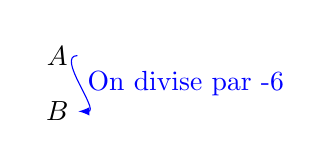
\begin{tikzpicture}% [every node/.style={anchor=west}]
  \matrix (n) [matrix of math nodes,
% row sep=0cm,column sep=0cm,  
%nodes={rectangle, draw},  
%    nodes in empty cells,
% column 1/.style={anchor=base east},
% column 3/.style={anchor=base west}%
]{
|(a)|A   \\
 \hbox to .1cm{}\\
|(b)|B   \\
};   
\draw[color=blue,->,>=latex] (a.east) to[out=180,in=0]node[midway,right] {\methode{On divise par -6}} (b) ;    
% \node[fit=(n-8-1)(n-8-3)]{$\mathcal{S} = \left\lbrace -1 \right\rbrace$};        
\end{tikzpicture}

\fi
\end{document}

